\label{gradience}

Much of the recent work in phonotactic theory has attempted to incorporate the intuition that phonotactic wellformedness is not an ``all-or-nothing'' matter.
Rather, it is alleged, wellformedness judgements have more fidelity than is implied by a simple contrast between ``possible'' and ``impossible'', and therefore must be measured and studied at a greater degree of granularity.

This is hardly a novel claim, though it has taken on greater import with the emergence of computational models of wordlikeness.
Early generative discussions of wordlikeness \citep[e.g.,][]{Chomsky1965,Halle1962} are best remembered for the famous examples [blɪk] and [bnɪk], the former representing a ``possible word'' of English and the latter representing an ``impossible word''. 
A naïve account of this contrast would be to derive it from the assumption that segments must be parsed into syllables or subject to further phonological repair (e.g., \citealt[10f.]{Hooper1973}, \citealt[57f.]{Kahn1976}, \citealt{Ito1989a}, \citealt[19f.]{Wolf2009}).
Unlike some languages (e.g., Morroccan Arabic: \emph{bniqa} `closet'), English does not permit stop-nasal onsets like [bn], so the latter nonce word cannot surface as such.
In other words, [bnɪk] is an impossible surface representation in English.
However, in \emph{The Sound Pattern of English} (henceforth, \emph{SPE}), \citet{SPE} introduce a third nonce word, [bznk], constructed so as to be even less English-like than [bnɪk].\footnote{
    That wordlikeness judgements depend on language-specific knowledge is apparent given that [bznk] is not impossible in all languages: Imdlawn Tashlhiyt Berber permits whole words consisting of a stop-fricative-nasal-stop sequence (e.g., [tzmt] `it is stifling'; \citealt[112]{Dell1985}). 
    This is clear evidence for the assumption that wordlikeness depends on language-specific knowledge.}
This leads \citeauthor{SPE} to conclude that wordlikeness intuitions are gradient.

\begin{quote}
Hence, a real solution to the problem of ``admissibility'' will not simply define a tripartite categorization of occurring, accidental gap, and inadmissible, but will define the `degree of admissibility' of each potential lexical matrix in such a way as to\ldots{}make numerous other distinctions of this sort (\emph{SPE}:416--417)
\end{quote}

This brings the theory of wordlikeness in line with the view of syntactic grammaticality presented by foundational documents like \emph{The Logical Structure of Linguistic Theory} \citep{LSLT} and \emph{Aspects of the Theory of Syntax} \citep{ASPECTS}, and reflexes can be found in later work, such as the proposals of \citet{BARRIERS} and \citet{Huang1982}; see \citealt[43f.]{Schutze1996} for a critique.

\citeauthor{SPE}'s claim about the gradient nature of phonotactic wellformedness does not seem to have had much of an impact on practices of the time---as can be seen from discussion in the previous chapter, contemporary critiques focused on other elements of the \emph{SPE} phonotactic theory---but reflexes can once again be found in later work: for instance, \citet{Borowsky1989}, \citet[50f.]{Clements1983}, and \citet{Myers1987} all assume a contrast between ``peripheral'' and absolutely ungrammatical sound sequences.

Recent discussions of gradient grammaticality in wordlikeness attempt to present experimental support for \citeauthor{SPE}'s intuitions:

\begin{quote}
When native speakers are asked to judge made-up (nonce) words, their intuitions are rarely all-or-nothing. 
In the usual case, novel items fall along a gradient cline of acceptability. \citep[][9]{Albright2009a}

In the particular domain of phonotactics gradient intuitions are pervasive: they have been found in every experiment that allowed participants to rate forms on a scale.
\citep[][382]{Hayes2008a}

A defect of current grammatical accounts of phonotactics is that they render simple up-or-down decisions concerning well-formedness and cannot account for gradient judgements. But when judgements are elicited in a controlled fashion from speakers, they always emerge as gradient, including all intermediate values. \citep[371]{Shademan2006}
\end{quote}

If the presence of intermediate values in wordlikeness tasks is evidence for the gradient nature of phonotactic wellformedness, then it follows that wordlikeness intuitions should be measured and modeled with a high degree of granularity.
For instance, this would be strong evidence against the naïve account of the [blɪk]-[bnɪk] contrast just alluded to, since it cannot easily be extended to account for ``numerous other distinctions''.
However, this chapter argues that there are both theoretical and empirical reasons to doubt the implicit hypothesis linking scalar wordlikeness ratings and gradient wellformedness.
First, intermediate ratings are characteristic of all gradient rating tasks, and therefore are irrelevant to the question of whether the internal phonotactic system is categorical or gradient.
Secondly, simple baselines better account for gradient well-formedness judgements than current computational models of phonotactic knowledge, suggesting that the gradience observed in these tasks do not derive from known grammatical mechanisms.

%are ``\ldots{}under the obligation to say why \emph{what it takes to be} data relevant to the confirmation of its theories \emph{are} data relevant to the confirmation of its theories'' \citep[200]{Fodor1981b}.

\section{Aspects of the theory of gradient grammaticality}

The aforementioned discussions of gradient aspects of wordlikeness judgements takes for granted that intermediate ratings are the product of an internal system of gradient grammaticality.
This view is itself an instance of what is known as \emph{common-sense} or \emph{naïve realism}; in the cognitive sciences, this often takes the form of the assumption that experimental data can be taken at face value, without mediation from other sources of information.
However, there are several arguments for \emph{a priori} skepticism about the (a) linguistic abilities required for reporting gradient grammaticality judgements, (b) intermediate acceptability ratings as evidence for gradient grammaticality, and (c) the total lack of previous attempts to consider categorical models of wellformedness.

\subsection{A model of gradient intuitions}

Current research into gradient wellformedness is concerned with specifying a function from sound sequences to scalar judgements, and thus describes the wellformedness system at a level of some abstraction, corresponding roughly to what \citet{Marr1982} calls the ``computational'' level of description.
This is only one part of any model of gradient grammaticality, however; further assumptions are needed to articulate the internal representations and algorithms by which this function computes.

First, consider the architecture which is implied by any system of gradient grammaticality.
It is essential that a system of gradient grammaticality have access to a relatively faithful representation of stimuli in a wellformedness task, and therefore it must be able to parse an enormous range of linguistic structures, including many which are not generated by the grammar itself; independent perception and production grammars may be necessary. 
A scalar value, representing wellformedness, must then be assigned to this parse.
To report wellformedness, the speaker must transform this scalar value in accordance with the numerical scale chosen by the experimenter.

Each step of this procedure merits scrutiny, however.
First, speakers have difficulty perceiving \citep{Berent2007a,Brown1956,Dupoux1999,Kabak2007a} and producing \citep{Davidson2005,Davidson2006a,Davidson2006b,Davidson2010,GallagherInPress,Rose2007,Vitevitch1998,Vitevitch2005} phonotactically illicit non-words, suggesting that speakers' ability to faithfully parse illicit representations is at best quite limited.
Secondly, the computation of a scalar value serves no further purpose than to provide for gradient well-formedness judgements, so an objection might be made here on evolutionary grounds.
It is quite mysterious why the human language endowment includes constraints on pronominal binding, for instance, but no one can doubt that these constraints are implicated in everyday language use; far more bizarre is the suggestion that the linguistic endowment includes mechanisms only implicated in certain experimental tasks.
Next, speakers must be able to consciously access and report the magnitude of this value (it must be \emph{cognitively penetrable} in the sense of \citealt{Pylyshyn1984}), an ability which is limited in many other domains.
Finally, there is some evidence that speakers do not (or perhaps, cannot) respect the numerical scales chosen by experimenters \citep{Sprouse2011}.

It is informative to compare this baroque model to the architecture implied by a binary well-formedness judgement.
When presented with a linguistic item in a judgement task, the grammar attempts to assign a parse. 
Speakers then access whether or not parsing was successful.
There are reasons to think that parsing of ungrammatical structures does in fact result in a ``crash'': whereas syntactic priming increases the acceptability of grammatical structures \citep{Luka2005}, ungrammatical structures show no priming effects \citep{Sprouse2007b}.
As priming of linguistic structures is thought to implicate shared representations in memory, this suggests different memory mechanisms for grammatical and ungrammatical linguistic objects.
%This cannot be reduced to the fact that ungrammatical structures fail to denote, since well-formed but non-existent structures do produce facilitory priming \citep[e.g.,][]{Longtin2005}. 
Finally, the fact that requests for repetition and clarification are ubiquituous in spontaneous speech illustrates further that speakers are frequently aware when parsing has failed.
Consequently, a great deal of evidence is needed to reject this simple model in favor of the gradient grammaticality architecture.

\subsection{What some linguistic intuitions might not be}

As first noted by \citet{Chomsky1963b}, speakers experience difficulty processing sentences with multiple center embeddings.
\citet{Gibson1999} perform a controlled experiment which reveals that speakers rate sentences like (\ref{gibson}a), which is well-formed, less grammatical than (\ref{gibson}b), despite the fact that a moment of reflection reveals that the latter sentence is nonsensical.

\begin{example}[A well-formedness illusion]
\label{gibson}
\begin{tabular}{l l@{}l}
a. &    & The patient who the nurse who the clinic had hired admitted met Jack. \\
b. & *  & The patient who the nurse who the clinic had hired met Jack. \\
\end{tabular}
\end{example}

\noindent
It is informative to consider that this well-known result has had no effect on the theory of syntactic representations, only on the theory of linguistic memory; it is recognized as the product of cognitive restrictions found in non-linguistic domains, as a \emph{task effect}.
This contrasts with the argument made by \citet{Hayes2000}, that gradient wordlikeness judgements demand a considerable and unmotivated revision to the grammatical architecture, as is discussed below.

The results of controlled experiments are often biased by subtle details that seem orthogonal to the task: for instance, certain types of duration judgements are systematically biased by consumption of caffeine \citep{Gruber2005}.
It should come as no surprise, then, that a highly salient aspect of a judgement task, the scale used for responses, also influences the results obtained.
\citet*{Armstrong1983} argue that rating tasks using many-valued scales may induce intermediate ratings as a task effect.

\citet{Armstrong1983} are concerned with experimental evidence for the nature of cognitive concepts.
While they do not attempt to dispute that certain concepts (e.g., \emph{fruit}) have a family-resemblance structure \citep[e.g.,][]{Rosch1975a}, they assert that it is apparent that other concepts are ``definitional'' (i.e., all-or-nothing), a notion which they illustrate with \emph{odd number}.

\begin{quote}
No integer seems to sit on the fence, undecided as to whether it is quite even, or perhaps a bit odd. No odd number seems odder than any other odd number. \citep[274]{Armstrong1983}
\end{quote}

\noindent
However, when subjects are asked to rate, using a 7-point Likert scale, how representative individual odd counting numbers are of the concept \emph{odd number}, they freely use intermediate ratings; the ratings they obtain with instances of \emph{odd number} and \emph{even number} are shown in Figure \ref{agg}.

\begin{figure}[t]
\centering
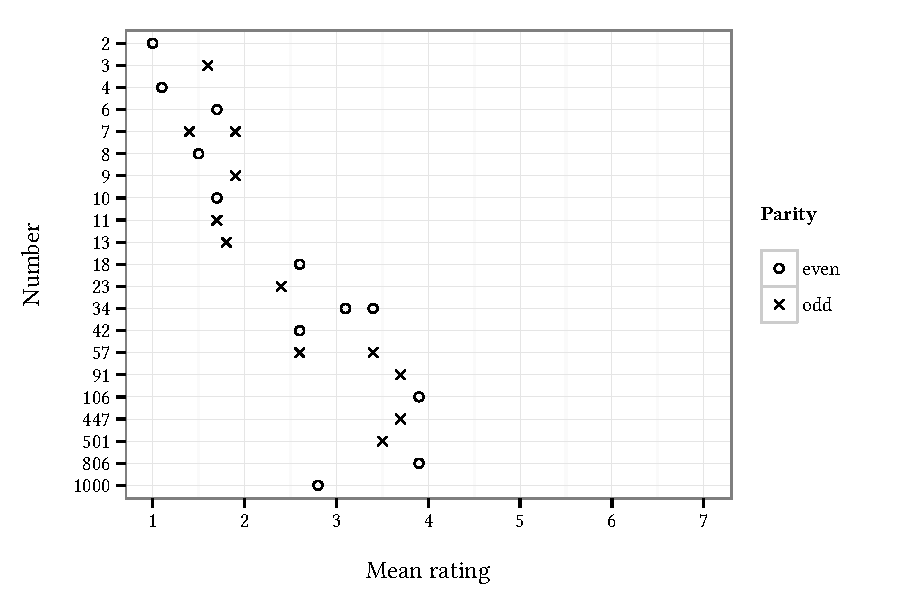
\includegraphics{agg.pdf}
\caption{Subjects freely use intermediate ratings when asked to rate how representative even and odd numbers were of ``even'' and ``odd'', respectively (\citealp{Armstrong1983}; ``1'' indicates ``most representative'')}
\label{agg}
\end{figure}

This suggests that the gradience observed is primarily an artifact of the task itself. 
\citeauthor{Schutze2011} suggests that the nature of this effect might be understood as the result of speakers' attempts to reconcile bizarre experimental tasks with their knowledge.

\begin{quote}
Putting it another way, when asked for gradient responses, participants will find some way to oblige the experimenter; if doing so is incompatible with the experimenter's actual question, they apparently infer that she must have really intended to ask something slightly different. \citep[24]{Schutze2011}
\end{quote}

As \citeauthor{Armstrong1983} observe, these results show that the scalar judgement tasks provide no evidence as to whether the category being rated is categorical or gradient.

\begin{quote}
\ldots{}we hold that \emph{fruit} and \emph{odd number} have different structures, and yet we obtain the same experimental outcome for both. But if the same result is achieved regardless of the concept structure, then the experimental design is not pertinent to the determination of concept structure. \citep[284--5]{Armstrong1983}
\end{quote}

It might be said that these results reveal something about the representation of odd numbers.
\citeauthor{Armstrong1983} anticipate this objection.

\begin{quote}
Some have responded to these findings very consistently, by asserting that the experimental findings are to be interpreted as before: that, psychologically speaking, odd numbers as well as birds and vegetables are graded concepts\ldots{} We reject this conclusion just because we could not explain how a person could compute with integers who believed that 7 was odder than 23. We assert confidently that the facts about subjects being able to compute and about their being able to give the definition of odd number, etc., are the more important, highly entrenched, facts we want to preserve and explain\ldots{} \citep[284]{Armstrong1983}
%we ourselves are prepared to give up the seeming fact that some odd numbers appear, as shown by their behavior in certain experimental paradigms, to be odder than others\ldots{}we do not give it up by saying that it was no fact; rather, by saying it must have been a fact about something other than the structure of concepts. \citep[284]{Armstrong1983}
\end{quote}

No scientist has risen to the challenge of constructing a theory that might account for the fact that 447 is rated more odd than 3, and as \citeauthor{Armstrong1983} suggest, it is unclear whether such a theory could preserve more central facts about oddness.
Here it is possible to draw an analogy to phonotactic theory.
According to current orthodoxy, the wellformedness of a sequence is closely related to its type frequency (i.e., frequency in the lexicon).
Is it then the case that [bl] is a significantly ``better'' onset than [kl], simply because the former is approximately twice as frequent, and if so, is it possible to also ensure that these sequences are treated the same with respect to syllabification?

\subsection{Evidencing gradience}

\citet{Hayes2000} argues that it is ``uninsightful'' to attribute gradience to task effects, insofar as these effects implicate grammatical representations. 

%\citep[?]{Hayes2000}
%``much of the patterning of gradient judgments is based on authentic structural aspects of the linguistic material being judged'' 

\begin{quote}
\ldots{}patterns of gradient well-formedness often seem to be driven by the very same principles that govern absolute well-formedness\ldots{} I conclude that the proposed attribution of gradient well-formedness judgments to performance mechanisms would be uninsightful. Whatever ``performance'' mechanisms we adopted would look startlingly like the grammatical mechanisms that account for non-gradient judgments. \citep[99]{Hayes2000}
\end{quote}

\noindent
The logic of this implication is indisputable.
However, there is little empirical support for the claims that absolute and gradient well-formedness derive from similar principles; indeed, there have been no prior attempts to evaluate categorical and gradient models of wordlikeness on an equal footing.
In light of the complexities of gradient models, such an evaluation requires strong quantitative evidence for the superiority of gradient grammatical models.
The evaluation below represents a first attempt to fill this gap.
%FIXME clements and keyser 

It is not that categorical models have been ignored by the literature on wordlikeness modeling, but rather that they have not been compared.
\citet{Frisch2000} and \citet{Vitevitch1997} find that speakers' wordlikeness ratings of multisyllabic words are correlated with a probabilistic measure of the well-formedness of the constituent syllables. 
Unfortunately, no attempt is made to control for the well-formedness of syllable contact clusters in these words: some of the stimuli have medial consonant clusters containing both voiced and voiceless obstruents (e.g., [ɡaɪbsaɪk]), something which is exceptionally rare in English simplex words (see \S\ref{ova}).
Similarly, \citet{Hayes2008a}, who compare their gradient model of wordlikeness against a set of English phonotactic constraints proposed by \citet{Clements1983}, first transform these constraints, several of which are without exception, into probabilities.
While this is consistent with their claim, that ``the ability to model gradient intuitions [is] an important criterion for evaluating phonotactic models'' \citep[382]{Hayes2008a}, little insight can be gained by annotating an exceptionless rule ``$p = 1.0$''. 
\citeauthor{Hayes2008a}'s principle precludes any attempt to test the hypotheses that underlies it, and therefore must be rejected.

% FIXME make this work: 
%(see \citealt{Sproat1993} and \citealt{Wrench2003} for articulatory investigations).

\section{Evaluation}
\label{2evaluation}

As \citet{Newmeyer2007} writes ``the idea that categoricity is not represented in the data itself is a truism. Whether distinctions of grammaticality (as opposed to acceptability) are binary is a difficult question.'' (398)
The mere presence of gradience in judgements cannot falsify the claim of gradient grammaticality; another method is needed to evaluate this claim.
As a first step towards a falsifiable theory of gradient wordlikeness, the remainder of this chapter considers intermediate ratings in gradient wordlikeness tasks are reliably predicted by the computational models that have been proposed.
If a model is incapable of accounting for intermediate ratings, there are two possibilities: either the model itself is improperly specified and therefore at fault, or the inputs and outputs of the model are unrelated to the actual causes of the intermediate ratings, \emph{contra} \citet{Hayes2000}.

It is plausible that speakers might differentiate, in a regular fashion, between different types of ``impossible'' words, and a gradient model should reliably predict the distinctions that speakers make.
There are also claims that speakers distinguish between different types of ``possible'' words, so that, for instance, [stɪn] \emph{stin} is rated more English-like than [blɪn] \emph{blin} \citep[e.g.,][]{Albright2009a}, because the former onset is more frequent in the English lexicon.
Even if wordlikeness judgements can be effectively modeled with a gross contrast between possible and impossible words, a gradient model might show a correlation with the residual ratings.
All of these possibilities are considered below.

\subsection{Materials}

This evaluation uses a large sample of three previously published studies on English wordlikeness comprising 125 subjects and 187 items.
Two criteria were used to select these three studies.
First, the stimuli must be presented aurally so as to eliminate any possibility of orthographic effects \citep[e.g.,][]{Berent2001b,Berent2008b}. 
Secondly, the data must be sufficiently ``phonotactically diverse'': that is, it must include both items like \emph{blick} and \emph{bnick}. 
This excludes studies like that of \citet{Bailey2001}, in which few if any items contain gross phonotactic violations of the type represented by \emph{bnick}.
In the absence of phonotactic violences, little variance in wordlikeness ratings can be attributed to phonotactic wellformedness, making it difficult to determine the coverage of gradient wellformedness models.
The data used here is summarized in Table \ref{counts}.

\begin{table}[t]
\centering
\begin{tabular}{l rrr}
\toprule
                           & subjects & items & trials \\
\midrule
\citeauthor{Albright2007}  & 68       & 40    & 2,720  \\
\citeauthor{Albright2003b} & 24       & 86    & 2,064  \\
\citeauthor{Scholes1966}   & 33       & 63    & 2,178  \\
\midrule
\textsc{Total}             & 125      & 187   & 6,962  \\
\bottomrule
\end{tabular}
\caption{Subject and item counts for the wordlikeness study}
\label{counts}
\end{table}

\subsubsection{\citealt{Albright2007}}

\citet{Albright2007} administers a wordlikeness task in which 68 adult speakers rate 40 monosyllabic nonce words, presented aurally, on a 7-point Likert scale with endpoints labeled  ``completely impossible as an English word'' and ``would make a fine English word''. 
\citeauthor{Albright2007}'s study is primarily concerned with the effects of different onset types (e.g., well-formed /bl/, marginal /bw/, unattested /bn, bd, bz/), and there is less diversity among the choice of rimes, none of which are obviously ill-formed.

\subsubsection{\citealt{Albright2003b} (norming experiment)}

\citet{Albright2003b} have 24 adult speakers rate 87 aurally presented monosyllabic nonce words on a 7-point Likert scale with endpoints labeled ``completely bizarre, impossible as an English word'' and ``completely normal, would make a fine English word''.
This task was administered to establish phonotactic norms for a later nonce word inflection task.
Their item [raɪf] is excluded in this study, since this is an actual word of English, \emph{rife}.
\citet{Albright2009a} uses this data to compare computational models of wordlikeness.

\subsubsection{\citealt{Scholes1966} (experiment 5)}

\citet{Scholes1966} conducts several wordlikeness tasks with students in 7th grade (approximately 12--13 years of age).
The data used here is his experiment 5, in which 33 speakers provide a ``yes'' or ``no'' as to whether each of the 63 items, presented aurally, are ``likely to be usable as a word of English''. 
Like the study by \citet{Albright2007}, the focus is on onset well-formedness and there is minimal diversity in rime type. 
Two items, [klʌŋ] \emph{clung} and [bɹʌŋ] \emph{brung} (a dialectal past participle of \emph{bring}), are excluded here as actual words of English. 
\citet{Albright2009a} and \citet{Hayes2008a} also use this data for the purposes of model evaluation; following \citet{Frisch2000}, they use the proportion of ``yes'' responses for each item so as to derive a continuous measure of well-formedness.

\subsection{Method}

Models are evaluated by comparing their scores to the average rating of each word using four correlation statistics. 
Each of these range between $[-1, 1]$, where $1$ indicates a perfect positive correlation and $-1$ denotes a perfect negative correlation. 
\citet{Hayes2008a} evaluate their model using the Pearson (``product-moment'') $r$, a parametric correlation measure.
It has long been argued \citep[e.g.,][]{Stevens1946} that parametric statistics are inappropriate for analysis of Likert scale data, like those used by \citet{Albright2007} and \citet{Albright2003b}, since the Pearson $r$ makes a \emph{linearity assumption}.
That is, it assumes that nonce words rated ``1'' and  ``3'', for instance, are just as different as are those rated ``4'' and ``6''. 
A weaker assumption, more appropriate for Likert scale data, is the \emph{monotonicity assumption}: that ``1'' is less English-like than ``3'', which is less English-like than ``4'', and so on.
However, it also has been claimed that $r$ is particularly robust to violations of the linearity assumption \citep[e.g.,][]{Havlicek1976}.
Pearson $r$ is reported here, but this should not be taken to imply an endorsement of its use for Likert scale data.

\citeauthor{Hayes2008a} also report Spearman $\rho$; this statistic requires only the weaker assumption of monotonicity, but it is difficult to give a simple interpretation to the coefficient.
Two other non-parametric statistics, the Goodman-Kruskal $\gamma$ and the Kendall $\tau_b$ are much easier to interpret, as follows \citep{Noether1981}. 
These statistics are computed by comparing every model score/wordlikeness rating pair to every other: a comparison is counted as \emph{concordant} if the greater of the two model scores is the one associated with the greater of the two wordlikeness ratings (that is, the model ranks these two nonce words in accordance with speakers' ratings), and as \emph{discordant} otherwise.
These two statistics differ only in the treatment of ``ties'', pairs where either the model score or wordlikeness rating are identical.
For $\gamma$, ties are ignored, and the coefficient is 

\begin{equation*}
\gamma = \displaystyle\frac{c - d}{c + d}
\end{equation*}

\noindent
where $c$ and $d$ represent the number of concordant and discordant pairs, respectively.
The $\tau_b$ statistic uses a similar formula, but also incorporates a penalty for ties in model score which are not also paired with ties in wordlikeness ratings, or vice versa.
\citet{Albright2009a} uses a variant of this statistic to evaluate wordlikeness models.

\subsection{Models}

The nonce word stimuli from these three studies are scored automatically using four computational models.
The first two models represent baselines for comparison to the latter two state-of-the-art gradient models.
The scores are reproduced in Appendix \ref{ratings}.

\subsubsection{Gross phonotactic violation}

A simple baseline is constructed by separating nonce words into those which contain a phonotactic violation and those which do not. 
As all nonce words here are monosyllabic, this task can be localized to two subcomponents of the syllable, the onset and the rime. 
This is not to imply that these are the only domains over which phonotactic violations might be stated, but there are prior claims that onset and rime are particularly important domains for stating phonotactic constraints (e.g., \citealt{Fudge1969}, \citealt{Kessler1997}, \citealt{Treiman2000}). 
Speakers are adept at separating syllables into these units \citep{Treiman1983,Treiman1986,Treiman1995}, and they are implicated by patterns of speech errors \citep{Fowler1987,Fowler1993}.

Operationalizing ``phonotactic violation'' is somewhat more difficult.
The simplest possible mechanism is chosen here: an onset or rime is identified as well-formed if it occurs with non-zero frequency in a representative sample, and is identified as ill-formed otherwise.
This is not to imply that all unattested onsets or rimes should be regarded as ill-formed, or that all onsets or rimes with non-zero frequency in this data are well-formed.
For instance, \citet{Albright2009a} judges [dɹɛsp] \emph{dresp} to be phonotactically well-formed, despite the total lack of [ɛsp] rimes in English; similar observations have been made concerning English onsets \citep[e.g.,][]{Cairns1972,Moreton2002}.

The representative sample used to define the phonotactic baseline is derived from those entries of the CMU pronunciation dictionary which occur at least once per million words in the SUBTLEX-US frequency norms; these norms are known to be particularly strongly correlated with other behavioral measures \citep{Brysbaert2009}.
These pronunciations are then syllabified, and individual syllables parsed into onset and rime, according to a process described in detail in Appendix \ref{syllabification}.

Wordlikeness ratings from the three studies are plotted against this gross contrast in Figure \ref{boxplot}.
While there are several outliers, there can be little doubt that gross phonotactic status accounts for a considerable amount of variance in wordlikeness judgements.

\begin{figure}[t]
\centering
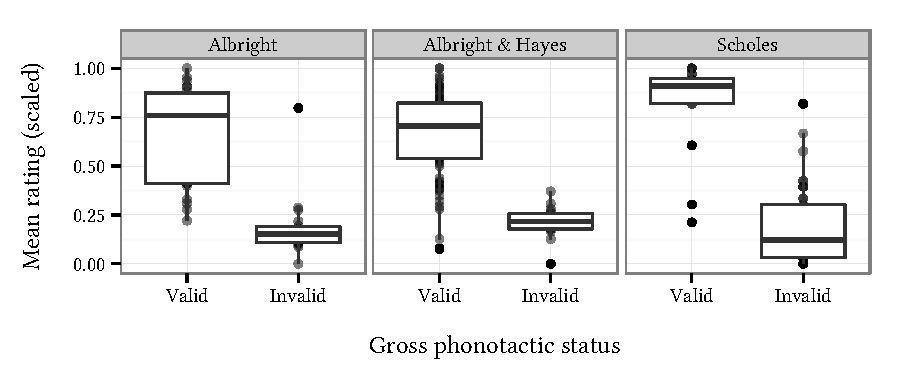
\includegraphics{boxplot.pdf}
\caption{Gross phonotactic status and item-averaged wordlikeness ratings}
\label{boxplot}
\end{figure}

\subsubsection{Lexical neighborhood density}

A second baseline is provided by measures of similarity to existing English words, which has long been applied to model wordlikeness judgements (e.g., \citealt{Bailey2001}, \citealt{Greenberg1964}, \citealt{Kirby2007}, \citealt{Ohala1986b}, \citealt{Shademan2006,Shademan2007}, \citealt{Vitevitch1998,Vitevitch1999a}). 
\citeauthor{LSLT} (\citeyear{LSLT}: 151, fn.~27) suggests that grammaticality judgements in general might be influenced by similarity to existing grammatical structures, and \citet[417f.]{SPE} outline a similarity-based wordlikeness model. 
More recently, it has been observed (e.g., \citealt[51]{Coleman1997}, \citealt{Hay2004a}) that nonce words which flagrantly violate English sonority restrictions but which bear common affixes (e.g., *\emph{mrupation}) are rated highly English-like.

A wide variety of lexical similarity measures were considered, including a variant of the Generalized Neighborhood model \citep{Bailey2001}, PLD20 \citep{Suarez2011}, and a set of measures provided by the Irvine Phonotactic Calculator \citep{Vaden2009}. 
The measure best correlated with wellformedness judgements is also the most venerable measure of lexical similarity: Coltheart's $N$ \citep{Coltheart1977}, which is defined as the number of words in some representative sample which can be changed into a target nonce word by a single insertion, deletion, or substitution of a phoneme.
\citet{Greenberg1964} find a correlation between wordlikeness ratings and a variant of this measure which only counts words differing by a single substitution.
This is plotted against ratings from the three studies in Figure \ref{neighborhood} with a superimposed local regression (LOESS; \citealt{Cleveland1988}) curve; neighborhood density accounts for much of the variance in ratings.

%The effects of neighborhood density in various psycholinguistic tasks are emergent properties of many models of speech production \citep[e.g.,][]{Luce1998,Luce2000} and perception \citep{Marslen-Wilson1984,Marslen-Wilson1987,McClelland1986,Norris1994,Norris2000}.

\begin{figure}[t]
\centering
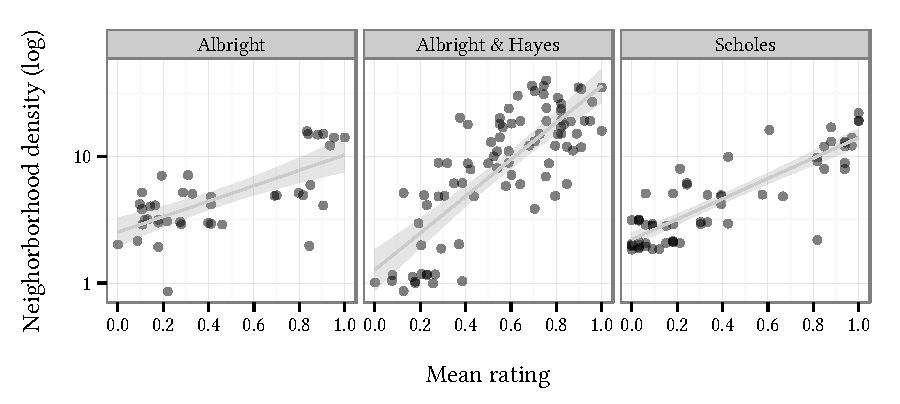
\includegraphics{neighborhood.pdf}
\caption{Correlation between Coltheart's $N$ and item-averaged wordlikeness ratings, with LOESS curve}
\label{neighborhood}
\end{figure}

While there is nothing inherently ``phonotactic'' about Coltheart's $N$, it indirectly incorporates much of the information present in the gross phonotactic baseline. 
Consider [blɪk]: since there is nothing marked about any part of this nonce word, a ``neighbor'' might be found by modifying any phone: e.g., \emph{click}, \emph{brick}, \emph{bloke}, \emph{bliss}. 
However, since [bn] onsets are unattested in English, a neighbor of [bnɪk] must somehow modify this cluster: this leaves only \emph{brick} and \emph{nick}. 
\citet{Bailey2001} and \citet{Frauenfelder1993} note that neighborhood density is also strongly correlated with measures like bigram probability, but it has been argued elsewhere that phonotactic measures and neighborhood density have distinct effects \citep[e.g.,][]{Berent2003,Pitt1998b,Vitevitch1998,Vitevitch1999a}.

\subsubsection{Segmental bigram probability}

Faciliatory effects of bigram probabilities (i.e., shorter latencies) are reported for other nonce word tasks conducted with adults, including single-word shadowing \citep{Vitevitch1997,Vitevitch1998}, same/different judgements \citep{Lipinski2005,Luce2001,Vitevitch1999a,Vitevitch2005}, and lexical decision \citep{Pylkkanen2002a}. 
\citet{Albright2009a} applies bigram probability as a model of wordlikeness judgements. 
The bigram probability of a sequence $ijk$, for instance, is defined as 

\begin{equation*}
\displaystyle \hat{p}(ijk) = p(i|\textsc{start}) \cdot p(j|i) \cdot p(k|j) \cdot p(\textsc{stop}|k)
\end{equation*}

\noindent
That is, it is the product of sequence-initial $i$, the probability of $j$ following $i$, the probability of $k$ following $j$, and the probability of the sequence ending after $k$.

\citet{Albright2009a} compares two variants of this model, the first operating over segments, the second over sets of features. 
Unfortunately, the latter model is not described in sufficient detail to allow it to be implemented directly, and there is no publicly available implementation.
However, \citeauthor{Albright2009a}'s evaluation, which includes the \citet{Scholes1966} and \citet{Albright2003b} data, finds an advantage for the segment-based model.
In implementing this model, it was found that a slight improvement could be made by preventing any phoneme-to-phoneme transition from having zero probability. 
This is accomplished by adding 1 to the count of every transition, a technique used in natural language processing and known as Laplace, or ``add one'', smoothing.
As can be seen in Table \ref{bigramcomparison}
this results in a slight increase in the correlation between the scores from this model and wellformedness ratings 
This smoothed segmental bigram score is adopted below.
In Figure \ref{bigram}, it is plotted against wordlikeness ratings from three studies.

\begin{table}[t]
\centering
\begin{tabular}{l rrrr}
\toprule
                                 & Pearson $r$ & Spearman $\rho$ & G-K $\gamma$ & Kendall $\tau_{b}$ \\
\midrule
featural  bigrams                &       {.71} &       {.64}     &       {.45}  &       {.45} \\
segmental bigrams                &       {.74} &       {.67}     &       {.48}  &       {.47} \\
segmental bigrams with smoothing & \uline{.75} & \uline{.70}     & \uline{.50}  & \uline{.50} \\
\bottomrule
\end{tabular}
\caption{Correlation between item-averaged wordlikeness ratings for the \citet{Albright2003b} norming study and three variants of bigram probability}
\label{bigramcomparison}
\end{table}

\begin{figure}[t]
\centering
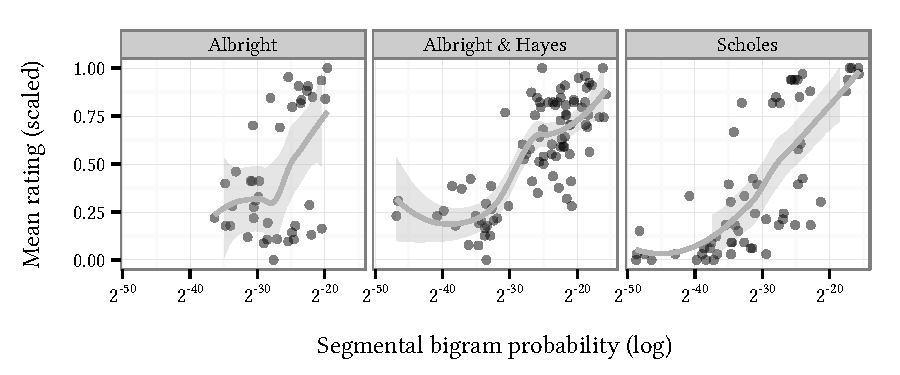
\includegraphics{bigram.pdf}
\caption{Correlation between smoothed segmental bigram score and item-averaged wordlikeness ratings, with LOESS curve}
\label{bigram}
\end{figure}

\subsubsection{Maximum entropy phonotactics}

\citet{Hayes2008a} present a model which uses the principle of maximum entropy to weigh a large number of competing phonotactic constraints (e.g., \citealt{Goldwater2003}, \citealt{Jager2007}). 
\citeauthor{Hayes2008a} use a complex method to evaluate their model. First, they extract onset sequences from the CMU pronunciation dictionary, and use these to train the model. 
The model is then used to score the onsets of the \citet{Scholes1966} nonce words. 
Then they compute a parameter for transforming their model scores so as to maximize the correlation between these transformed scores and wordlikeness ratings, then report the resulting correlation.\footnote{
    This is contrary to standard practices in natural language processing, in that the data used for evaluation is also used to fit the model (namely, the transformation's parameter); when this is the case, there is reason to suspect the parameter values will not generalize to new data.
    No transformation is used here; this only has an effect on the Pearson $r$ coefficient, since they use a transformation that preserves monotonicity.}
\citet{Albright2009a} reports that the maximum entropy model, training and testing only on onsets, performs well on the \citet{Scholes1966} data, but does not generalize well to the \citet{Albright2003b} sample.
Consequently, the model was trained to score whole words, not just onsets, using the subset of the CMU dictionary described above.

Since this model has numerous experimenter-defined parameters, a close replication of \citeauthor{Hayes2008a}'s original paper is attempted: both their implementation and phonological feature specifications are used here.
Following \citet{HayesInPress}, dictionary entries are syllabified using the procedure described in Appendix \ref{syllabification}, and a novel feature [$\pm$\textsc{Coda}] is added to allow the model to distinguish coda and onset consonants.
Also, following \citeauthor{Hayes2008a}, constraints are limited to those spanning as many as three segments and an ``accuracy schedule'' of [$.001$, $.01$, $.1$, $.2$, $.3$] is used.
Since the maximum entropy model produces slightly different scores on each run, the worst-performing of 10 runs is reported here, following \citeauthor{Hayes2008a}.
The resulting scores are plotted against wordlikeness ratings in Figure \ref{maxent}; it can be seen that the model assigns the highest possible score to a large variety of nonce words, though many words with a low rating receive the highest MaxEnt probability score.
It appears that this model is still not robust enough to reliably extracting phonotactic generalizations from monosyllabic words.

\begin{figure}[t]
\centering
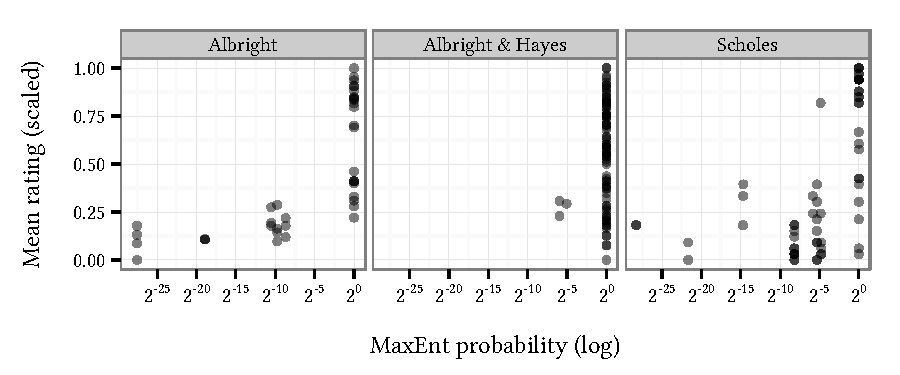
\includegraphics{maxent.pdf}
\caption{Correlation between MaxEnt score and item-averaged wordlikeness ratings}
\label{maxent}
\end{figure}

\subsection{Results}

Table \ref{scores} displays the full set of correlation coefficients, for each of the three data sets, and for each of the four models. 
The first observation is that in general, there is a positive correlation between model score and ratings in each pair. 
The two baselines, gross phonotactic status and neighborhood density, are by far the strongest models across statistics and studies, with gross phonotactic status performing the strongest under the Goodman-Kruskal $\gamma$ and on the \citet{Albright2007} data, and neighborhood density performing strongly under nearly all other statistics and data sets. 

\begin{table}[t]
\centering
\begin{tabular}{l rrr c rrr c rrr c rrr}
\toprule
              &         \multicolumn{3}{c}{Pearson $r$} &&     \multicolumn{3}{c}{Spearman $\rho$} && \multicolumn{3}{c}{G-K $\gamma$} && \multicolumn{3}{c}{Kendall $\tau_b$} \\
\cmidrule{2-4} \cmidrule{6-8} \cmidrule{10-12} \cmidrule{14-16}
              &           A &         AH &            S &&           A &       AH    &           S &&           A &          AH &           S &&           A &          AH & S \\
\midrule
Gross status & \uline{.73} &       {.60} &       {.80} && \uline{.82} &       {.66} &       {.80} && \uline{.87} & \uline{.93} & \uline{.91} &&       {.67} &       {.47} &       {.62} \\
Density ($N$) &       {.67} & \uline{.79} & \uline{.86} &&       {.61} & \uline{.74} & \uline{.82} &&       {.49} &       {.57} &       {.74} &&       {.45} & \uline{.56} & \uline{.67} \\
Bigram $p$ &       {.46} &       {.75} &       {.74} &&       {.34} &       {.70} &       {.79} &&       {.25} &       {.50} &       {.63} &&       {.25} &       {.50} &       {.61} \\
MaxEnt $p$ &       {.70} &       {.21} &       {.53} &&       {.66} &       {.39} &       {.58} &&       {.85} &       {.61} &       {.56} && \uline{.68} &       {.16} &       {.48} \\ 
\bottomrule
\end{tabular}
\caption{Correlation between item-averaged wordlikeness ratings and model scores}
%; the largest coefficient for each statistic/data set pair is underlined.}
\label{scores}
\end{table}

It is also possible to consider whether there is any residual correlation between bigram and MaxEnt model scores, and wordlikeness ratings within the ``valid'' and ``invalid'' groups defined by the gross phonotactic status measure. 
Kendall $\tau_{b}$ correlations within these subgroups for each data set are shown in Table \ref{resid}. 
The only reliable positive correlation is present among the ``valid'' items as rated by the smoothed segmental bigram model. 
This model is somewhat capable of accounting for contrasts between different ``possible'' nonce words: for instance, it favors [plin] \emph{plean} over [brɛlθ] \emph{brelth} just as subjects in the \citet{Albright2007} study do; this can also be seen in the top three panels of Figure \ref{bigramresid}.
Within the set of ``invalid'' items, however, neither grammatical model reliably distinguishes among items; both models, for instance, rate [ptʌs] \emph{ptus} more well-formed than [bnʌs] \emph{bnus}, but speakers have the opposite preference.

\begin{table}[t]
\centering
\begin{tabular}{l rrr c rrr}
\toprule                
             & \multicolumn{3}{c}{``Valid'' items} && \multicolumn{3}{c}{``Invalid'' items} \\
\cmidrule{2-4} \cmidrule{6-8}
             %& \multicolumn{3}{c}{Kendall $\tau_{b}$} && \multicolumn{3}{c}{Kendall $\tau_{b}$} \\
             &         A &       AH &        S &&     A  &       AH &          S \\
\midrule
Bigram score &     {.65} &    {.34} &    {.60} &&    {.03} & {$-$.17} &    {.47} \\
MaxEnt score &     {.00} & {$-$.15} & {$-$.32} && {$-$.42} &    {.29} & {$-$.16} \\
\bottomrule
\end{tabular}
\caption{Kendall $\tau_{b}$ correlation between model scores and item-averaged wordlikeness ratings, sorted according to gross phonotactic status}
\label{resid}
\end{table}

\begin{figure}[t]
\centering
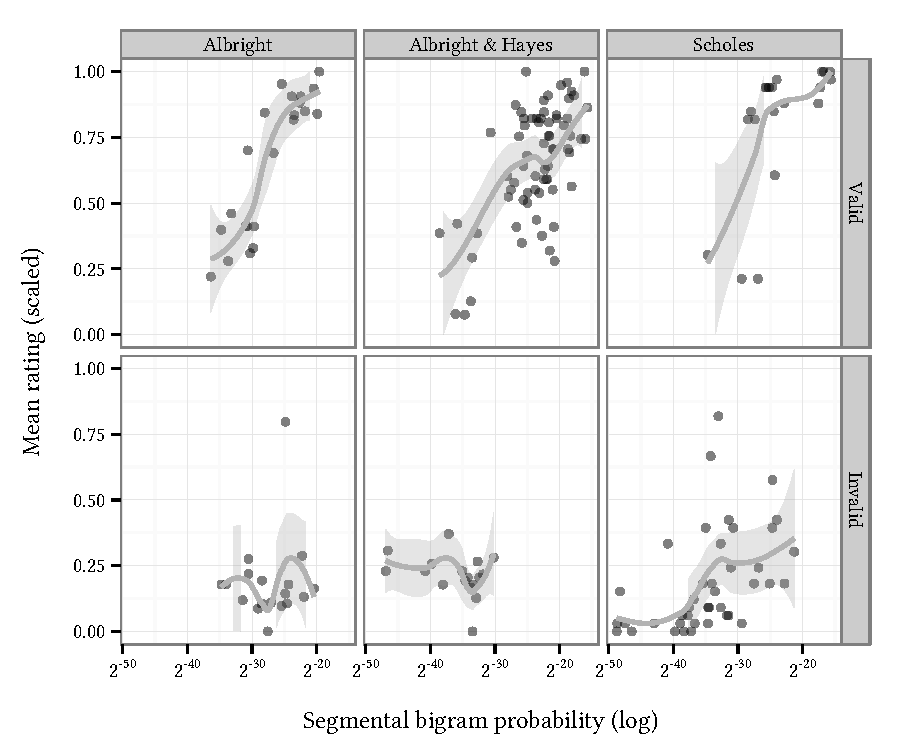
\includegraphics{bigramresid.pdf}
\caption{Correlation between smoothed segmental bigram score and item-averaged wordlikeness ratings, sorted according to the gross phonotactic status, with LOESS curve}
\label{bigramresid}
\end{figure}

\subsection{Discussion}

The bigram and MaxEnt models do not reliably outperform simple baselines. 
From this it can be inferred that the gradient models do not reliably predict intermediate ratings. 
Nor do these models reliably distinguish within classes of ``valid'' and ``invalid'' words in a way that conforms with wordlikeness ratings.

A serious limitation of this evaluation is the primitive nature of the gross phonotactic status baseline. 
It does not allow for any way to state constraints on onset-nucleus sequences, which have been proposed for some languages (e.g., \citealt{Kirby2007} on Cantonese), or constraints spanning whole syllables \citep[e.g.,][]{Berkley1994b,Berkley1994a,Clements1983,Coetzee2008b,Fudge1969}.\footnote{
    It is disputed whether English in particular exhibits onset-nucleus restrictions.
    \citet{Clements1983} claim that ``cooccurrence restrictions holding between the nucleus and preceding elements of the syllable appear to be just as common as cooccurrence restrictions holding between the nucleus and following elements'' (20), but admit that at least some of these generalizations may represent accidental gaps.
    However, \citet{Kessler1997}, argue there are no clear restrictions on English onset-nuclei pairs.}
Furthermore, the gross phonotactic baseline does not have any mechanism for generalizing the wellformedness of [ɛsp] rimes from \emph{clasp}, \emph{lisp}, and other rimes consisting of a lax vowel followed by [sp] found in English, but \citet{Borowsky1989}, for instance, proposes a theory of possible rimes in English which makes the correct prediction regarding [ɛsp].
This is not embedded in an acquisitional model, but many models of syllable type acquisition have been proposed \citep[e.g.,][]{Fikkert1994,Levelt2000,Pan2003,Pan2004}.
As observed by \citet{Smith1973} in a careful study of a single child acquiring English, children's productions are at first highly restricted but progress systematically to stages with fewer and fewer restrictions.
Assuming productive competence is an appropriate measure of syllable acqusition, this suggests that syllable types are acquired like many other linguistic phenomena in that the child progresses from subset to superset.
The difficulty here is that the typology of syllables must be delineated so that, for instance, the robust presence of [æsp] and [ɪsp] implies acceptance of [ɛsp].

The gross phonotactic baseline could also be extended so as to recognize more than two levels of wellformedness, without introducing the infinite amount of contrast implied by fully gradient models.
While the bigram and MaxEnt models do not appear to be able to reliably distinguish intermediate levels of well-formedness, it might be desirable to encode the intuition that, for example, [ʒlɪk] \emph{zhlick}, is more English-like than [bnɪk], though both have unattested onsets \citep[e.g.,][50f.]{Clements1983}.
It is also possible to imagine that phonotactic violations would have a cumulative effect on well-formedness. For instance, a nonce word with an unattested onset and an unattested rime, like [tsɪlm], might be less English-like than either [tsɪl] or [sɪlm], an ability that could easily be extended to the gross phonotactic baseline.
Cumulativity effects are predicted by the bigram and MaxEnt models, among others \citep[e.g.,][]{Albright2008,Anttila1997}, but could easily be incorporated into a simple baseline by counting the number of violations.
However, as of yet there is no convincing evidence for cumulativity effects in wordlikeness tasks, and the stimuli used here are not suited to test this hypothesis.

\section{Conclusions}

State-of-the-art computational models of wellformedness do not reliably predict intermediate ratings in wordlikeness tasks.
To the degree to which the bigram or MaxEnt models are correlated with speakers' judgements, these judgements are more precisely modeled by similarity to existing words, or by a gross contrast between attested and unattested onsets and rimes. 
While it remains an open question whether future gradient models will account for intermediate judgements, the current evidence suggests that gradient grammaticality is not crucial for modeling gradient wordlikeness judgements.
This does not imply that wordlikeness judgements collected using Likert scales or magnitude estimation are tainted; \citet{SprouseSubmitted} argue that gradient wellformedness measures are better able to detect syntactic violations thought to be categorical than are binary judgements, and it seems likely this result would also hold for wordlikeness tasks.
However, intermediate ratings can no longer be taken at face value.

%\citep{Bard1996}
%FIXME short discussion of the utility of gradient judgements in syntax
%\citep[e.g.,][]{Hale2003c,Hale2006,Levy2008,Roark2009}
%\citet{Pereira2000}

%An emerging consensus suggests, however, that infants attend to transitional probabilities primarily in the absence of grammatical cues \citep{Gambell2005,Hohne1994,Johnson2001,Jusczyk1999c,Lignos2012b,Mattys2001a,Shukla2007,Lew-Williams2012}. The vacuous nature of current evidence for gradient phonotactic knowledge in adults further weakens any hypothesis that would link statistical learning in infants to adults' behaviors.
%Using the head-term preference paradigm, \citet{Jusczyk1993b} and \citet{Friederici1993} find that typically-developing children as young as 9 months of age distinguish between nonce words which are and are not phonotactically valid in their target language. \citet{Jusczyk1994} report that 9-month-old children acquiring English also show preferences for nonce words with high positional probability over those with low positional probability. 
%``Suppose that linguistic well-formedness really is an all-or-nothing matter, but that the judgments we get are filtered through various performance mechanisms. It is the performance mechanisms, not the grammar itself, which results in the gradient intuitions. If this is so\ldots{}we should be reducing them (somehow) to two categories and developing a model of the judgment process itself to account for the numbers observed.''
